\section{Adobe XD}
\setauthor{Raffeiner Christine}
\begin{wrapfigure}{r}{0.3\textwidth}
    \begin{center}
      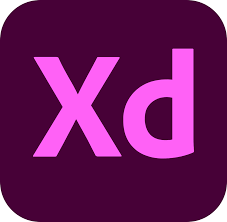
\includegraphics[width=0.15\textwidth]{pics/XD_Logo.png}
    \end{center}
\end{wrapfigure}
Adobe XD ist eine kostenpflichtige vektorbasierte Design-Plattform für die Erstellung von Wireframes, Animations- und Interaktions-Design, 
User Interface Design und Prototypen und gilt weiters als All-in-One-Tool. Adobe XD erlaubt es Komponenten als eine Art Template anzulegen 
und diese zur Wiederverwendung und Synchronisierung gängiger Elemente wie zum Beispiel Buttons und Navigationssymbole zu verwenden.
Verändert man nun eine erstellte Hauptkomponente im Nachhinein, werden alle zugehörigen Änderungen automatisch in allen Instanzen angezeigt.
Mit Komponentenzuständen können allerdings Variationen für eine einzelne Komponente erstellt werden. Zum Beispiel kann eine andere 
Hintergrundfarbe im Hover-Zustand (Mauszeiger liegt über dem Element) bestimmt werden.
\newline
\newline
Eine weitere Funktion Responsive Resize erkennt Layouts und passt das Design für andere Formate automatisch an. Adobe XD bietet ebenfalls die Verwendung von Plug-ins für 
die verschiedensten Funktionen, wie zum Beispiel die Verwendung von Icons, an. Um einen funktionierenden Prototyp zu erstellen 
kann auf die Verwendung von Ankerlinks nicht verzichtet werden, da nahtlose Übergänge und eine Navigation von Seite zu Seite dafür unabdinglich sind. \cite{noauthor_adobe_nodate}, \cite{noauthor_was_nodate}

\section{Oracle SQL-Developer}
\setauthor{Raffeiner Christine}
\label{chap:sqldeveloper}
Oracle SQL Developer ist eine kostenlose, integrierte Entwicklungsumgebung, für die 
Entwicklung und Verwaltung von Datenbanken. SQL Developer bietet eine vollständige 
Ende-zu-Ende-Entwicklung von PLSQL- und SQL-Anwendungen, ein Arbeitsblatt für die Ausführung von 
Abfragen und Skripten, eine Datenbankadministrationskonsole für die Verwaltung der Datenbank, eine 
Berichtschnittstelle und eine vollständige Datenmodellierungslösung den Data Modelers. \cite{noauthor_was_nodate-1}

\subsection{Data Modeler}
Oracle SQL Developer Data Modeler ist ein kostenloses, grafisches Tool, 
dass die Datenmodellierungsaufgaben vereinfacht. 
Mit dem Data Modeler können Benutzer/innen logische, relationale, physische und 
mehrdimensionale Datentypenmodelle erstellen, durchsuchen und bearbeiten. 
Der Data Modeler bietet Forward- und Reverse-Engineering-Funktionen und unterstützt die 
gemeinsame Entwicklung durch integrierte Quellcodekontrolle. \cite{noauthor_data_nodate}